\documentclass[12pt]{report}
\usepackage[utf8]{inputenc}
\usepackage[russian]{babel}
\usepackage[14pt]{extsizes}
\usepackage{listings}
\usepackage{graphicx}
\usepackage{amsmath,amsfonts,amssymb,amsthm,mathtools} 
\usepackage{pgfplots}
\usepackage{filecontents}
\usepackage{float}
\usepackage{indentfirst}
\usepackage{eucal}
\usepackage{enumitem}
%s\documentclass[openany]{book}
\frenchspacing

\usepackage{titlesec}
\titleformat{\section}
{\normalsize\bfseries}
{\thesection}
{1em}{}
\titlespacing*{\chapter}{0pt}{-30pt}{8pt}
\titlespacing*{\section}{\parindent}{*4}{*4}
\titlespacing*{\subsection}{\parindent}{*4}{*4}

\usepackage{indentfirst} % Красная строка

\usetikzlibrary{datavisualization}
\usetikzlibrary{datavisualization.formats.functions}

\usepackage{amsmath}

\usepackage{amssymb}

% Для листинга кода:
\lstset{ %
	language=lisp,                 % выбор языка для подсветки (здесь это С)
	texcl=true,
	extendedchars=\true,
	basicstyle=\small\sffamily, % размер и начертание шрифта для подсветки кода
	numbers=left,               % где поставить нумерацию строк (слева\справа)
	numberstyle=\tiny,           % размер шрифта для номеров строк
	stepnumber=1,                   % размер шага между двумя номерами строк
	numbersep=5pt,                % как далеко отстоят номера строк от подсвечиваемого кода
	showspaces=false,            % показывать или нет пробелы специальными отступами
	showstringspaces=false,      % показывать или нет пробелы в строках
	showtabs=false,             % показывать или нет табуляцию в строках
	frame=single,              % рисовать рамку вокруг кода
	tabsize=2,                 % размер табуляции по умолчанию равен 2 пробелам
	captionpos=t,              % позиция заголовка вверху [t] или внизу [b] 
	breaklines=true,           % автоматически переносить строки (да\нет)
	breakatwhitespace=false, % переносить строки только если есть пробел
	escapeinside={\#*}{*)},  % если нужно добавить комментарии в коде
	%inputencoding=utf8x,
	%extendedchars=\true
}



\usepackage[left=2cm,right=2cm, top=2cm,bottom=2cm,bindingoffset=0cm]{geometry}
% Для измененных титулов глав:
\usepackage{titlesec, blindtext, color} % подключаем нужные пакеты
\definecolor{gray75}{gray}{0.75} % определяем цвет
\newcommand{\hsp}{\hspace{20pt}} % длина линии в 20pt
% titleformat определяет стиль
\titleformat{\chapter}[hang]{\Huge\bfseries}{\thechapter\hsp\textcolor{gray75}{|}\hsp}{0pt}{\Huge\bfseries}


% plot
\usepackage{pgfplots}
\usepackage{filecontents}
\usetikzlibrary{datavisualization}
\usetikzlibrary{datavisualization.formats.functions}

\begin{document}
	\begin{titlepage}
	\newgeometry{pdftex, left=2cm, right=2cm, top=2.5cm, bottom=2.5cm}
	\fontsize{12pt}{12pt}\selectfont
	\noindent \begin{minipage}{0.15\textwidth}
		
\includegraphics[width=\linewidth]{pictures/b_logo.jpg}
	\end{minipage}
	\noindent\begin{minipage}{0.9\textwidth}\centering
		\textbf{Министерство науки и высшего образования Российской Федерации}\\
		\textbf{Федеральное государственное бюджетное образовательное учреждение высшего образования}\\
		\textbf{«Московский государственный технический университет имени Н.Э.~Баумана}\\
		\textbf{(национальный исследовательский университет)»}\\
		\textbf{(МГТУ им. Н.Э.~Баумана)}
	\end{minipage}
	
	\noindent\rule{18cm}{3pt}
	\newline\newline
	\noindent ФАКУЛЬТЕТ $\underline{\text{«Информатика и системы управления»}}$ \newline\newline
	\noindent КАФЕДРА $\underline{\text{«Программное обеспечение ЭВМ и информационные технологии»}}$\newline\newline\newline\newline\newline\newline\newline
	
	
	\begin{center}
		\Large\textbf{Отчет по лабораторной работе №4}\newline
	\end{center}
	
	\noindent\textbf{Название} $\underline{\text{~Моделирование системы массового обслуживания~~~~~~~~~}}$\newline\newline\newline
	\noindent\textbf{Дисциплина} $\underline{\text{~Моделирование~~~~~~~~}}$\newline\newline
	\noindent\textbf{Студент} $\underline{\text{Золотухин А. В.~~~~~~~~~~~~~~~~~~~~~~~~~~~~~~~~~~~~~~~~~}}$\newline\newline
	\noindent\textbf{Группа} $\underline{\text{ИУ7-74Б~~~~~~~~~~~~~~~~~~~~~~~~~~~~~~~~~~~~~~~~~~~~}}$\newline\newline
	\noindent\textbf{Оценка (баллы)} $\underline{\text{~~~~~~~~~~~~~~~~~~~~~~~~~~~~~~~~~~~~~~~~~~~~~~~~~}}$\newline\newline
	\noindent\textbf{Преподаватель}$\underline{\text{~Рудаков И. В.~~~~~~~~~~}}$\newline
	
	\begin{center}
		\vfill
		Москва~---~\the\year
		~г.
	\end{center}
 \restoregeometry
\end{titlepage}

	\anonsection{Условие лабораторной работы}
Требуется реализовать ПО, позволяющее генерировать алгоритмическим методом последовательность случайных чисел и проверять итоговую последовательность на случайность по любому критерию.
Также нужно добавить пользователю возможность генерировать последовательность из однозначных чисел и реализовать генерацию табличным методом.

\anonsection{Теоретическая часть}
В этом разделе будет приведено описание методов генерации последовательности случайных чисел и описан критерий проверки последовательности на случайность.

\subsection*{Виды генераторов случайных чисел}
Всего можно выделить четыре типа генераторов случайных чисел:
\begin{enumerate}
	\item \textbf{Аппаратные генераторы} используют результаты определённых физических процессов для создания требуемой последовательности. Аппаратный генератор случайных чисел состоит из источника энтропии и устройства, преобразующего значения, полученные с источника энтропии, в нужный формат.
	
	К такому типу относятся генераторы, основанные на фотоэффекте или тепловом шуме при работе полупроводникового диода. 
	На выходе получается последовательность, обладающая значительной степенью случайности, но у таких генераторов есть два недостатка: системы трудно реализовать в жизни, а процессов, позволяющие преобразовать энтропию в последовательность.
	
	\item \textbf{Алгоритмические генераторы} основаны на фиксированных алгоритмах, которые, в зависимости от некоторых физических параметров (например, содержимого ввода/вывода), выдают нужный результат. Подобные алгоритмы имеют программную реализацию и используются в коммерческом ПО.
	
	\item \textbf{Табличные генераторы} принимают на вход уже готовую последовательность, обладающую свойством случайности, после чего проводит различные манипуляции с ней (комбинирование, перемешивание), и выдают результат.
	К недостаткам этого подхода можно отнести лишнее использование памяти, предопределённость значений и ограниченность последовательности.
\end{enumerate}


\subsection*{Выбранный критерий определения случайности}
В качестве критерия был выбран критерий серий.

Пусть $l_n$ --- медиана наблюдаемых случайных величин. Каждому элементу выборки поставлен в соответствие знак ``+'' или ``-'' в зависимости от того больше он медианы или меньше. Пусть $n_1$ --- число плюсов, а $n_2$ --- число минусов. Серией называется последовательность из одинаковых знаков, ограниченная противоположными. Статистикой критерия является число серий $n$. Критическая область определяется неравенствами $n \le N_1$ и $n \ge N_2$, которые определяются из таблицы при малых значениях $n_1+n_2$. 


\begin{figure}[H]
	\centering
	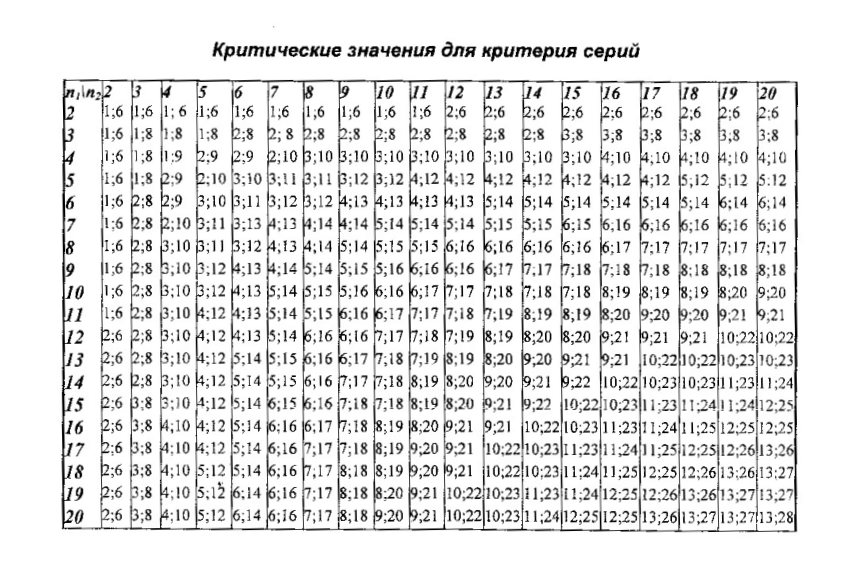
\includegraphics[width=1\linewidth]{inc/serial-table}
	\label{fig:serial-table}
\end{figure}`

Если $\max(n_1, n_2) \ge 20$, то

\[z_B=\frac{|n - \frac{2n_1n_2}{n_1+n_2} - 1| - \frac{1}{2}}{\sqrt[]{\frac{2n_1n_2(2n_1n_2-(n_1+n_2))}{(n_1+n_2)^2(n_1+n_2+1)}}} \sim N(0,1)\]
критическая область определяется неравенством 
\[z_B \le U_{\frac{\alpha}{2}} \text{	или	} z_B \ge  U_{1 - \frac{\alpha}{2}}\]

\section*{Демонстрация работы программы}

В ходе выполнения программы пользователю доступно меню, в котором он может выбрать размер последовательности, который нужно сгенерировать, уровень значимости, а также файл, если он хочет также проверить собственную последовательность.

На рисунке представлена демонстрация работы программы:

\captionsetup{justification=centering}
\begin{figure}[H]
	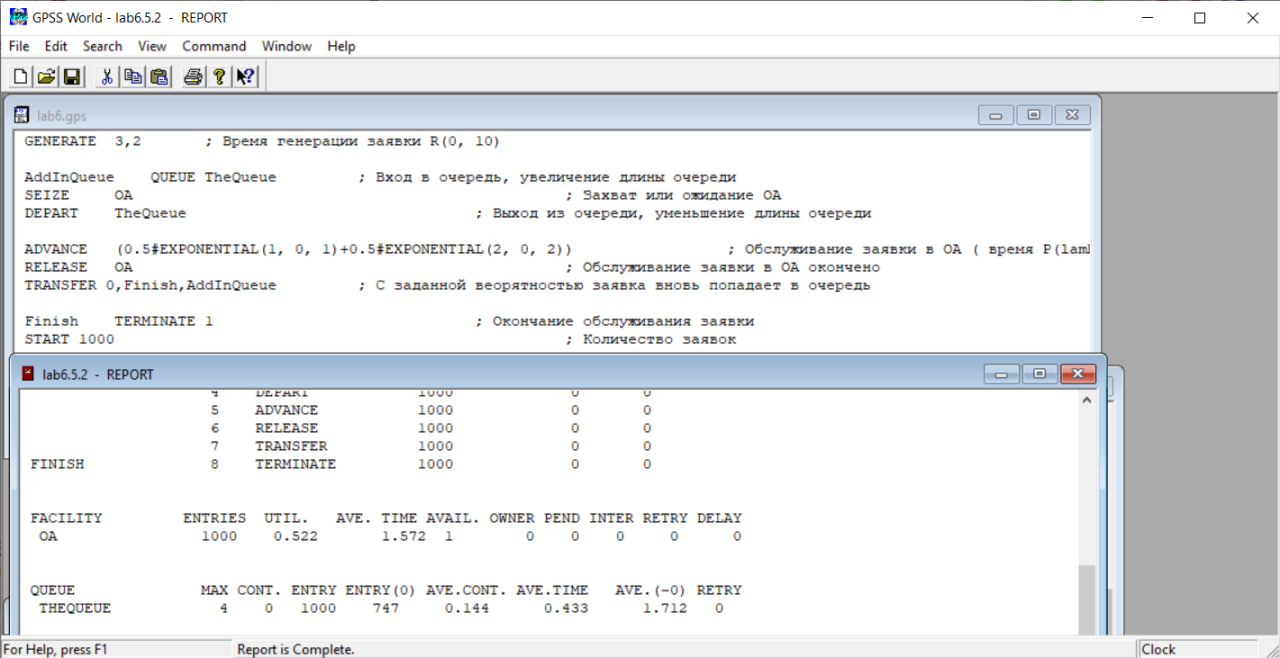
\includegraphics[width=\linewidth]{inc/demo}
	\centering
	\caption{Демонстрация работы программы}
\end{figure}



\end{document}